\documentclass[11pt,a4paper,openany]{report}
\usepackage[T1]{fontenc}
\usepackage[utf8]{inputenc}
\usepackage{lmodern}
\usepackage{microtype}
\usepackage{amsmath,amssymb,amsthm,mathtools,bm}
\usepackage{booktabs,array,longtable,tabularx}
\usepackage{xcolor}
\usepackage[margin=24mm,headheight=23pt]{geometry}
\usepackage{enumitem}
\usepackage{fancyhdr}
\usepackage{fancyvrb}
\usepackage{graphicx}
\usepackage{url}
\usepackage{xurl}
\usepackage{hyperref}

\definecolor{finblue}{HTML}{1F5A99}
\definecolor{fingreen}{HTML}{19733A}
\definecolor{finorange}{HTML}{D55E00}
\definecolor{finred}{HTML}{A61B1B}
\definecolor{finviolet}{HTML}{6A3D9A}

\hypersetup{
  unicode=true,
  colorlinks=true,
  linkcolor=finblue,
  citecolor=fingreen,
  urlcolor=finblue,
  pdftitle={FIN Programs 125--137: Trace Selection, Natural Localizers, Fractional Physics, and Operational Sources},
  pdfauthor={Krzysztof Żuchowski},
  pdfsubject={Invariant trace obstruction, natural C12 localizer, fractional dynamics, dimensional calibration, apparatus tomography, and signed operational sources},
  pdfkeywords={FIN, trace selection, cyclic groups, fractional Laplacian, stable process, wave dynamics, operational physics, apparatus tomography}
}

\pagestyle{fancy}
\fancyhf{}
\fancyhead[L]{\small FIN Programs 125--137}
\fancyhead[R]{\small Release 10.13}
\fancyfoot[C]{\thepage}
\setlength{\parindent}{0pt}
\setlength{\parskip}{0.55em}
\setlist{nosep,leftmargin=2em}
\setcounter{tocdepth}{2}
\setcounter{secnumdepth}{3}
\emergencystretch=3em

\newcommand{\one}{\bm 1}
\newcommand{\C}{\mathbb C}
\newcommand{\R}{\mathbb R}
\newcommand{\Z}{\mathbb Z}
\newcommand{\statusProven}{\textcolor{fingreen}{[Proven]}}
\newcommand{\statusComputer}{\textcolor{fingreen}{[Proven, computer-assisted]}}
\newcommand{\statusStrong}{\textcolor{finblue}{[Strong evidence]}}
\newcommand{\statusConditional}{\textcolor{finorange}{[Conditional]}}
\newcommand{\statusRefuted}{\textcolor{finred}{[Refuted in scope]}}
\newcommand{\statusOpen}{\textcolor{finviolet}{[Open]}}

\begin{document}
\hypersetup{pageanchor=false}
\begin{titlepage}
\centering
\vspace*{9mm}
{\Large\bfseries FIN Research Monograph --- Release 10.13\par}
\vspace{11mm}
{\Huge\bfseries FIN Programs 125--137\par}
\vspace{6mm}
{\Large Trace Selection, Natural Localizers,\\
Fractional Physics, and Operational Sources\par}
\vspace{17mm}
{\Large Krzysztof \.Zuchowski\par}
\vspace{2mm}
{\normalsize Independent Researcher --- Fractal Information Theory Project\par}
\vspace{2mm}
{\normalsize ORCID: \href{https://orcid.org/0009-0002-0909-3613}{0009-0002-0909-3613}\par}
\vspace{10mm}
{\large 27 July 2026\par}
{\normalsize Publication --- Preprint; record version 1.0.0\par}
\vfill
\begin{minipage}{0.88\textwidth}
\small
\textbf{Scope.} Thirteen executed studies of invariant trace selection,
the natural \(C_{12}\) localizer, quantitative fractional limits,
wave ultraviolet resolution, physical calibration, apparatus tomography,
parameter-source falsification, conditional damping completion, and signed
operational states.

\medskip
\textbf{Central result.} The localized fibre is natural, but its invariant
probability traces form a simplex. The uniform trace gives \(9/5\), while the
normalized Hilbert trace gives \(17/9\). Present symmetry does not select the
strict damping exponent.

\medskip
\textbf{Guardrail.} No strict selector, internal physical units, completed
legacy--strict bridge, role transfer, role-bearing \(L_{\mathrm{total}}\),
Theory-of-Everything closure, or external validation is claimed.

\medskip
\textbf{License.} Creative Commons Attribution 4.0 International (CC BY 4.0).
\end{minipage}
\vfill
\end{titlepage}
\hypersetup{pageanchor=true}

\pagenumbering{roman}
\chapter*{Publication statement}
\addcontentsline{toc}{chapter}{Publication statement}
This release reports Programs 125--137 and recommends Programs 138--150.
Proofs, computer-assisted calculations, strong numerical evidence,
conditional constructions, falsified candidates, and open obligations are
kept separate.

\tableofcontents
\clearpage
\pagenumbering{arabic}

\section{Confidence convention}

Every conclusion is labelled by one of the following standards.

\begin{itemize}
\item 
\textbf{Proven:} an analytic or finite mathematical argument is supplied.

\item 
\textbf{Proven, computer-assisted:} a finite computation is reproducible and covered by regression tests.

\item 
\textbf{Strong evidence:} analytic truncation control is combined with ordinary floating-point computation, but not machine-verified interval arithmetic.

\item 
\textbf{Conditional:} the conclusion is exact after a premise not presently sourced by strict FIN is added.

\item 
\textbf{Refuted in scope:} the stated candidate fails a specified necessary test.

\item 
\textbf{Open:} the required source, theorem, or empirical input is absent.

\end{itemize}

A numerical identity is not called a source theorem merely because it equals a frozen FIN parameter. A physical prediction is not claimed without a calibration map, an instrument model, and admitted external observations.

\section{Abstract}

This monograph executes thirteen research programs that continue the constructive analysis of FIN after Programs 113--124. The previous round built a homological--character fibre over the strict finite carrier,

\[
\mathcal F_p
=
\widetilde H_0(\ker m_p)\oplus\mathcal X_p^-,
\]

with dimension vector

\[
(1,2,2,2,2).
\]

Its uniform sector average is \(9/5\), suggesting the strict damping exponent. The first task of the present round is to determine whether that average is actually canonical.

The answer is negative. Even after granting the enlarged abstract symmetry \(\operatorname{Aut}(U(12))\cong S_3\), which permutes the three nonidentity unit elements, the five prime sectors split into three orbits,

\[
\{2\},\qquad \{3\},\qquad \{5,7,11\}.
\]

Consequently every invariant probability trace has the form

\[
w=(x,y,z/3,z/3,z/3),
\qquad x+y+z=1,
\]

and the induced exponent is

\[
\eta(w)=2-x.
\]

The value \(9/5\) requires \(x=1/5\) and is not selected by invariance. Moreover, the normalized Hilbert trace, arguably the most immediate dimension-weighted choice, gives

\[
\eta_{\rm Hilb}
=
\frac{1^2+4\cdot2^2}{1+4\cdot2}
=\frac{17}{9},
\]

not \(9/5\). This is a new trace-selection obstruction.

A positive result accompanies the obstruction. The fibre assignment is upgraded to a presentation-independent finite-carrier localizer. For every cyclic-group isomorphism \(\psi\),

\[
\psi\circ m_p=m_p\circ\psi,
\]

so the kernel homology and real-character component are transported naturally. The vector \((1,2,2,2,2)\) is therefore not an artefact of choosing a generator of \(C_{12}\). What remains absent is not the localizer but the state or trace placed on its sector algebra.

The fractional operator analysis is also strengthened. An FFT with analytic tail and frequency-cell bounds encloses every frequency in

\[
10^{-3}\le |q|\le2\cdot10^{-2}.
\]

The maximum conservative relative-remainder upper bound around the \(|q|^{4/5}\) law is \(2.2647\%\). The result is strong evidence rather than a formal interval theorem because the FFT itself uses guarded ordinary floating-point arithmetic. Finite-step characteristic functions are then compared quantitatively with the symmetric \(4/5\)-stable limit.

For wave dynamics, the same fractional generator produces a unitary \(L^2\) group, but the usual cutoff-free dispersive construction encounters an ultraviolet obstruction. On a dyadic shell of scale \(\Lambda\), the standard curvature estimate grows as

\[
t^{-1/2}\Lambda^{3/5}.
\]

It is not summable over ultraviolet shells. Thus a bandwidth or detector-resolution object is not optional if pointwise wave records are to be defined by this route.

The smallest external physical calibration is constructed explicitly:

\[
x_{\rm phys}=\ell x,\qquad
t_{\rm phys}=\tau t,\qquad
H_{\rm phys}=\frac{\hbar}{\tau}A.
\]

The logarithmic dimension matrix has rank three. Hence the dimensionless operator cannot internally determine length, time, and action merely by a change of notation; three independent calibrations are required unless a new dimensionful source theorem is added.

The round also constructs a finite-memory apparatus-tomography estimator, an exact projective crossover flow, an amplitude quotient, a trace-parameterized damping completion, and a signed operational receiver. The receiver detects opposite currents in prepared Fourier branches \(k\) and \(-k\), but it does not choose either branch. Therefore QW-2191 remains open.

The deepest surviving conclusion is precise. FIN now has a natural finite carrier localizer and a quantitatively supported fractional operational generator. Its principal missing theoretical object is a distinguished state on the localized sector algebra, together with an independently sourced calibration and preparation law. Symmetry, arithmetic coincidence, and state-dependent readout do not supply those objects.

\par\medskip\hrule\medskip

\chapter{Part I --- Scope, notation, and guardrails}

\section{Research questions}

Programs 125--137 address the following questions.

\begin{enumerate}
\item 
Does invariance select the trace producing \(\eta=9/5\)?

\item 
Can the fibre formula be made independent of a presentation of \(C_{12}\)?

\item 
Can the fractional symbol law be controlled on a continuum of frequencies rather than at selected sample points?

\item 
Can finite-step convergence toward the stable process be bounded quantitatively?

\item 
Does fractional wave evolution define pointwise records without a UV resolution?

\item 
What is the minimum calibration object needed to interpret the dimensionless operator physically?

\item 
Can apparatus memory be learned without assuming a parametric hidden model?

\item 
Is the local-to-fractional crossover governed by an exact projective flow?

\item 
Can the frozen phase and frequency be sourced by the new finite object?

\item 
Does quotienting amplitude clarify the role of \(\alpha_{\rm geo}\)?

\item 
How much of the legacy-to-strict damping bridge becomes exact after the trace is exposed as a variable?

\item 
Can an operational state produce the missing signed selector?

\item 
Is any external dataset presently admitted into this research chain?

\end{enumerate}

\section{Kernel split}

The two kernels are kept distinct:

\[
K_{\rm legacy}(d)
=
\alpha_{\rm geo}
\frac{\cos(\omega_{\rm L}d+\phi_{\rm L})}
{1+\beta_{\rm tors}d},
\]

\[
K_{\rm strict}(d)
=
\frac{\cos(\omega d+\phi)}
{1+\beta d^\eta}.
\]

The legacy kernel is an intermediate bridge object. It is not silently substituted for the strict kernel, and strict damping is not used to transport legacy physical-role formulas. A valid completion must separately account for amplitude, phase, frequency, nonlinear damping, certified topological data, and role preservation.

\section{Ontological and selector boundary}

Within the repository ontology, the nadsoliton is primordial fractal information in a solitonic state. No information layer below it is introduced here. This statement does not itself define an experimental preparation, physical clock, dimensional scale, or measurement instrument.

The finite orientation obstruction QW-2191 is respected. A signed observable is not a selector if its sign is inherited from a prepared branch. A strict selector would have to produce the branch or orientation without placing the desired sign in its premise.

\section{Strict lattice object}

For the fractional calculations, the positive jump weights are

\[
a_d=
\frac{|\cos(\omega d+\phi)|}{1+d^{9/5}},
\qquad
Z=2\sum_{d\ge1}a_d,
\]

and

\[
p_{\pm d}=\frac{a_d}{Z}.
\]

The Markov generator is \(I-P\) and the continuum candidate is

\[
C(-\Delta)^{2/5}.
\]

This positive jump object is used only in the stochastic/\allowbreak{}fractional lane. It does not replace the signed strict kernel in amplitude and bridge comparisons.

\par\medskip\hrule\medskip

\chapter{Part II --- Programs 125--126: the fibre, its naturality, and the missing trace}

\section{Program 125 --- Classification of invariant traces}

\subsection{Sector algebra}

The Program-122 fibres have dimensions

\[
d=(d_2,d_3,d_5,d_7,d_{11})=(1,2,2,2,2).
\]

The simplest commutative algebra recording the five sectors is

\[
\mathcal A_{\mathcal F}\cong\mathbb C^5.
\]

A probability trace on this algebra is a vector

\[
w=(w_2,w_3,w_5,w_7,w_{11}),
\qquad
w_p\ge0,\quad\sum_p w_p=1.
\]

The proposed exponent readout is

\[
\eta(w)=\sum_p w_p d_p=2-w_2.
\]

\subsection{Symmetry scopes and orbits}

There are two symmetry scopes that must not be conflated. Changes of generator of \(C_{12}\) commute with every \(m_p\) and therefore fix every prime label individually. Under carrier naturality alone, the full probability simplex remains admissible.

For a stronger falsification test, grant the full abstract automorphism group of \(U(12)\cong C_2\times C_2\). It is isomorphic to \(S_3\) and permutes the three nonidentity unit elements \(5,7,11\), while the exceptional nonunit primes \(2\) and \(3\) remain distinguished by kernel homology. A trace invariant under this enlarged symmetry must and may have the form

\[
w(x,y,z)
=
(x,y,z/3,z/3,z/3),
\]

where \(x,y,z\ge0\) and \(x+y+z=1\).

This proves that the invariant state space is a two-simplex. On it,

\[
\eta=2-x,
\qquad 1\le\eta\le2.
\]

In particular,

\[
\eta=\frac95
\quad\Longleftrightarrow\quad
x=\frac15.
\]

Even this enlarged invariance condition does not force \(x=1/5\). The weaker carrier-natural symmetry leaves still more freedom.

\subsection{Uniform and Hilbert traces}

Two natural-looking choices disagree:

\[
w_{\rm unif}=(1/5,1/5,1/5,1/5,1/5),
\qquad
\eta(w_{\rm unif})=\frac95,
\]

whereas weighting sectors by their Hilbert dimensions gives

\[
w_{\rm Hilb}
=
\frac1{9}(1,2,2,2,2),
\]

and

\[
\eta(w_{\rm Hilb})
=
\frac{17}{9}.
\]

The discrepancy is not a numerical defect. It is a mathematical demonstration that "take the natural trace" is under-specified.

\begin{figure}[htbp]
\centering
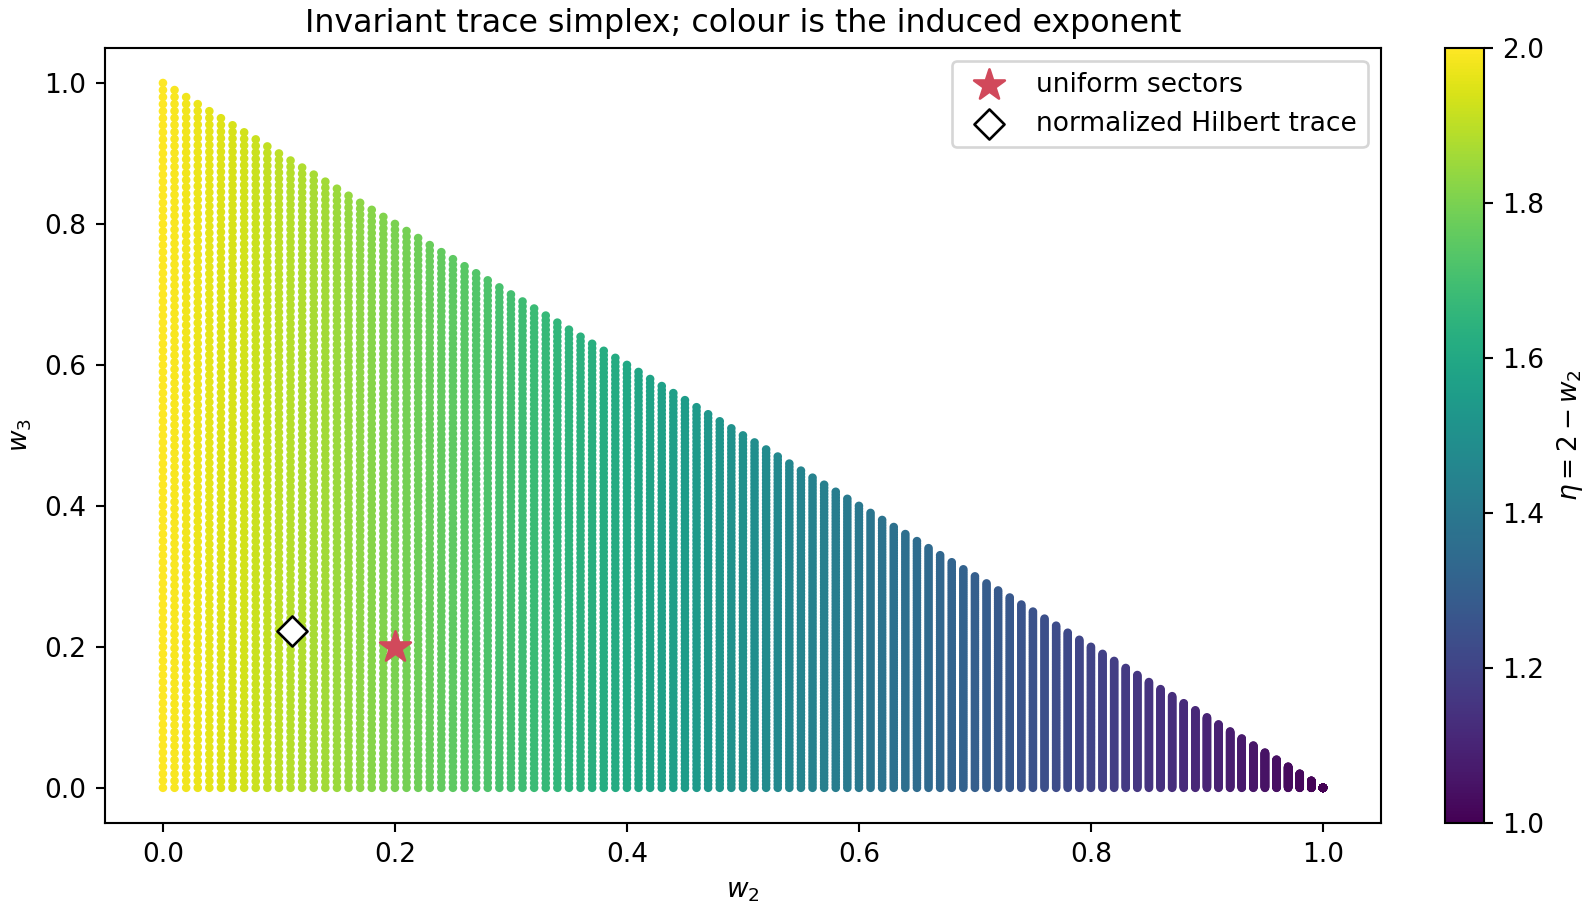
\includegraphics[width=0.94\textwidth]{FIN_Programs_125_137_Trace_Localizer_Physics_Figures/program125_invariant_trace_simplex.png}
\caption{Invariant trace simplex. Symmetry leaves two independent state parameters and does not select the uniform sector trace.}
\end{figure}

\textbf{Result:} \textbf{Proven.} Enlarged \(\operatorname{Aut}(U(12))\) invariance classifies a two-simplex of admissible traces and does not select \(\eta=9/5\). Carrier naturality alone permits the full simplex, so the no-go is robust to the symmetry scope.

\textbf{Falsification consequence:} any future derivation of \(9/5\) must supply a state-selection principle stronger than invariance. Maximum entropy would select the uniform trace only after the reference measure and admissible constraint set are specified; those are new premises, not consequences of the present fibre dimensions.

\section{Program 126 --- A natural finite-carrier localizer}

\subsection{Definition}

Let \(C_n\) be a finite cyclic group and let \(p<n\) be prime. Define

\[
m_p:C_n\longrightarrow C_n,
\qquad
m_p(x)=px.
\]

Let \(\mathcal X_p^-\) denote the direct sum of real-character lines on which evaluation at the unit \(p\) is negative. When \(p\) is not a unit, set that summand to zero. Then define

\[
\mathcal F_p(C_n)
=
\widetilde H_0(\ker m_p)
\oplus\mathcal X_p^-.
\]

\subsection{Naturality theorem}

For every cyclic-group isomorphism \(\psi:C_n\to C_n'\),

\[
\psi(px)=p\psi(x),
\]

hence

\[
\psi\circ m_p=m_p\circ\psi.
\]

It follows that \(\psi\) maps \(\ker m_p\) isomorphically to the corresponding kernel and induces an isomorphism of reduced zeroth homology. Conjugation also transports the real-character representation. Thus \(\mathcal F_p\) is presentation-independent at the cyclic-carrier level.

For \(C_{12}\) the decomposition is

\[
\begin{array}{c|cc|c}
p & \dim\widetilde H_0(\ker m_p) & \dim\mathcal X_p^- &
\dim\mathcal F_p\\
\hline
2&1&0&1\\
3&2&0&2\\
5&0&2&2\\
7&0&2&2\\
11&0&2&2
\end{array}
\]

All four changes of cyclic generator by the units \(1,5,7,11\) preserve the construction.

\begin{figure}[htbp]
\centering
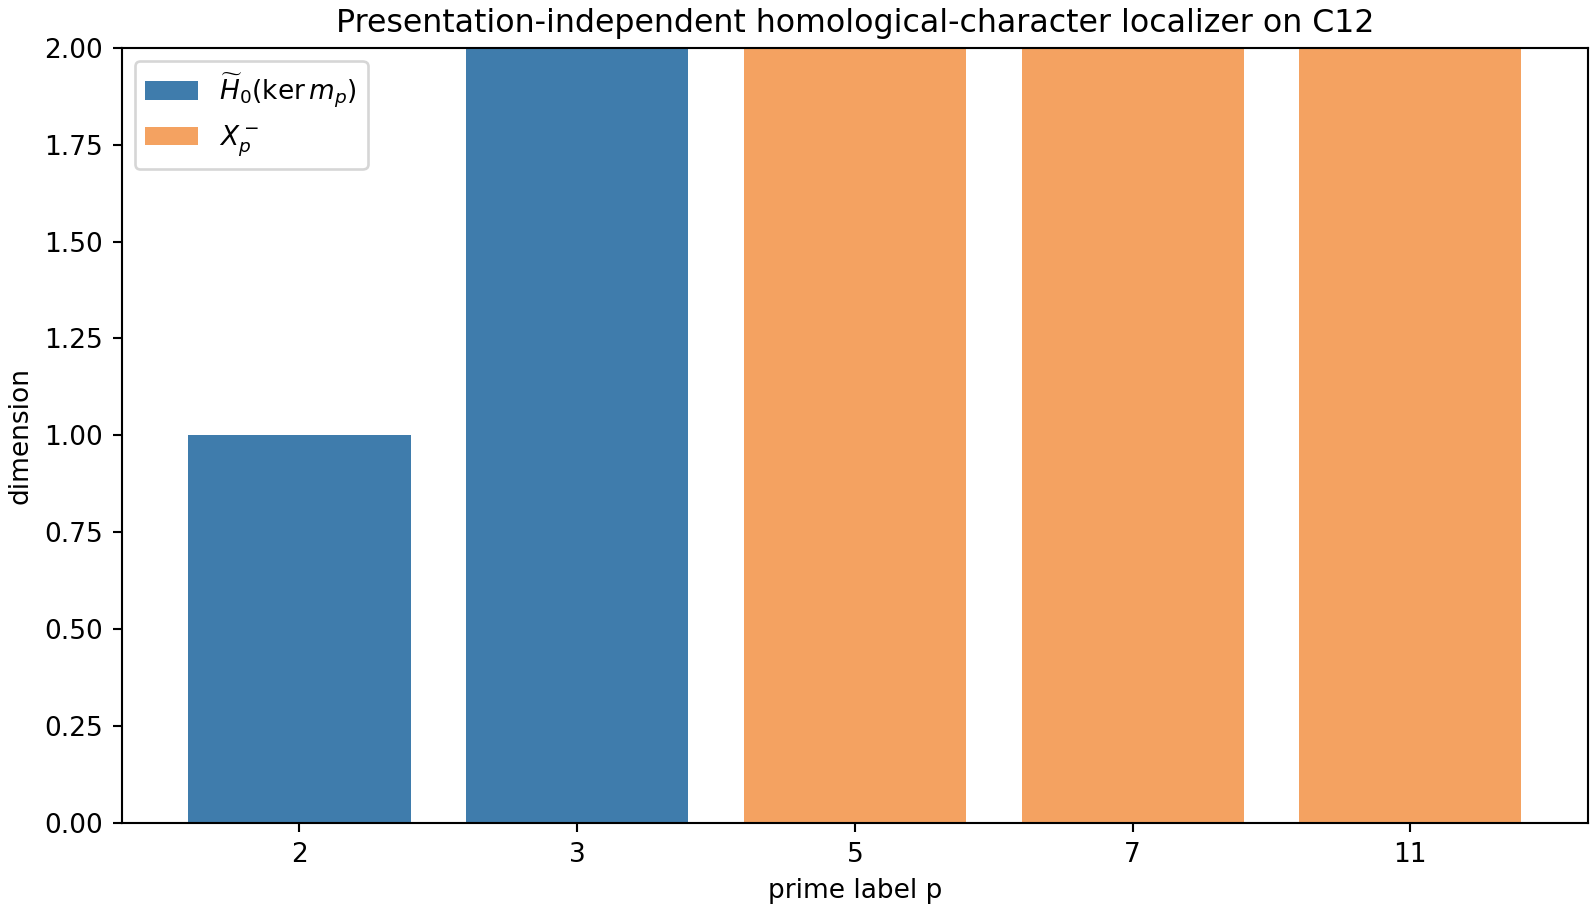
\includegraphics[width=0.94\textwidth]{FIN_Programs_125_137_Trace_Localizer_Physics_Figures/program126_natural_fibre_localizer.png}
\caption{Natural decomposition of the \(C_{12}\) homological--character fibres.}
\end{figure}

\textbf{Result:} \textbf{Proven.} A natural localizer exists once the strict \(C_{12}\) carrier is given.

\textbf{Open boundary:} the construction does not prove that the ontology sources that carrier, does not select a probability trace on the five sectors, and does not couple the trace to the strict damping law. The localizer closes a presentation defect, not the state-selection problem.

\par\medskip\hrule\medskip

\chapter{Part III --- Programs 127--129: quantitative fractional dynamics}

\section{Program 127 --- Continuous finite-window fractional enclosure}

\subsection{Fourier representation}

The normalized symbol is

\[
S(q)=1-\widehat p(q)
=
\frac{2\sum_{d\ge1}a_d(1-\cos qd)}{Z}.
\]

The Abelian candidate is

\[
S(q)\sim C|q|^{4/5}.
\]

Unlike a pointwise sample, a continuous-window certificate must control frequency cells, truncation tails, normalization, and numerical evaluation.

\subsection{Computation and analytic bounds}

The computation uses an FFT of length

\[
N=2^{21},
\]

retaining distances through

\[
D=1,048,575.
\]

For a cell of half-width \(\delta q=\pi/N\), the finite numerator varies by at most

\[
\delta q\,
2\sum_{d=1}^{D}a_d d.
\]

The omitted normalization is bounded by the monotone tail

\[
2\sum_{d>D}d^{-9/5}
\le
\frac{2D^{-4/5}}{4/5}.
\]

The numerator tail uses \(0\le1-\cos(qd)\le2\). These inequalities enclose every cell whose centre lies in the stated window.

\subsection{Result}

There are 6,338 covered frequency cells. The largest conservative relative remainder upper bound is

\[
0.0226460484.
\]

\begin{figure}[htbp]
\centering
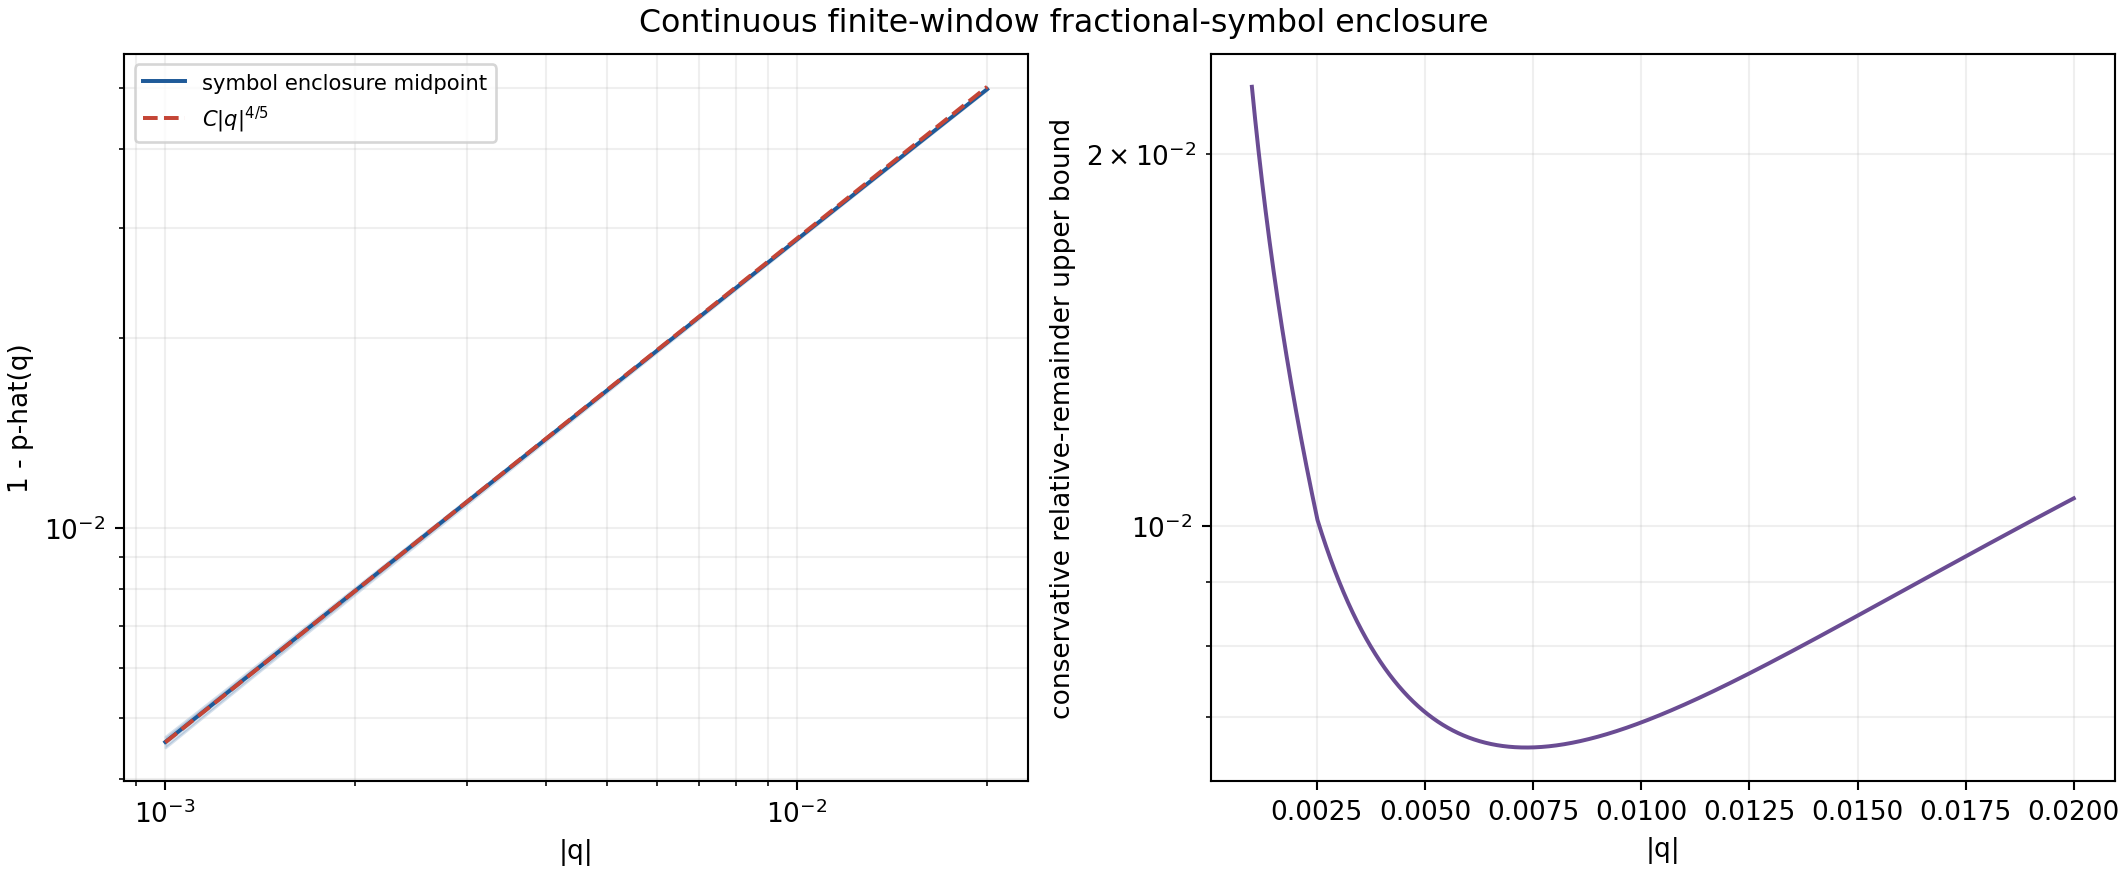
\includegraphics[width=0.94\textwidth]{FIN_Programs_125_137_Trace_Localizer_Physics_Figures/program127_continuous_fractional_enclosure.png}
\caption{Continuous finite-window enclosure around the \(C|q|^{4/5}\) symbol law.}
\end{figure}

\textbf{Result:} \textbf{Strong evidence with analytic tail and cell bounds.} The full compact window is covered, but the FFT is not performed in directed machine-verified interval arithmetic. A formal theorem would require replacing the guarded floating-point transform by a validated FFT or exact transform enclosure.

\textbf{What is not proved:} this finite window is not a rate theorem as \(q\to0\). Oscillatory tails and small divisors can become relevant below the window.

\section{Program 128 --- Quantitative stable finite-step window}

For a rescaled \(n\)-step process, set

\[
q_n=k\,n^{-5/4}.
\]

The finite characteristic function is

\[
\Phi_n(k)
=
\left(1-S(q_n)\right)^n,
\]

while the stable target is

\[
\Phi_\infty(k)=e^{-C|k|^{4/5}}.
\]

Program 127 provides lower and upper values of \(S\) and \(C\), and hence explicit intervals for both functions. Fifteen \((n,k)\) combinations lie inside the certified frequency window. Across them, the largest endpoint-distance bound is

\[
8.7262\times10^{-3},
\]

and the largest strict separation of the two conservative intervals is

\[
4.9583\times10^{-3}.
\]

\begin{figure}[htbp]
\centering
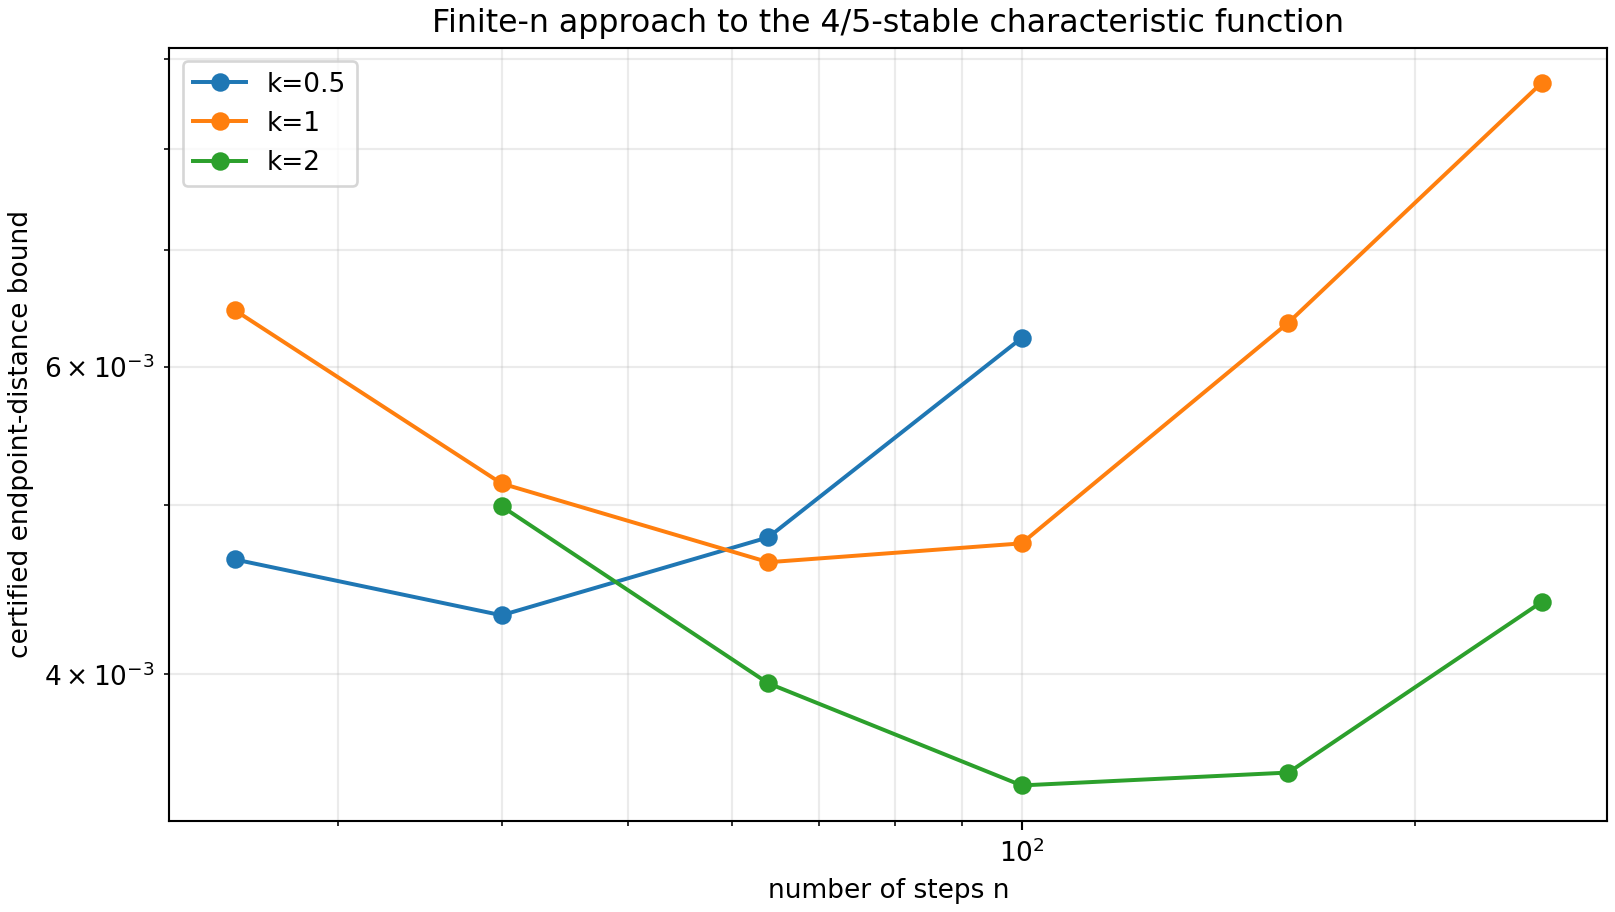
\includegraphics[width=0.94\textwidth]{FIN_Programs_125_137_Trace_Localizer_Physics_Figures/program128_quantitative_stable_window.png}
\caption{Finite-step characteristic-function distance bounds in the certified frequency window.}
\end{figure}

\textbf{Result:} \textbf{Conditional quantitative theorem.} The bounds are valid conditional on the Program-127 enclosure. They demonstrate the scale of the finite-step correction but do not monotonically improve throughout the table, because the smallest \(q\) cells have looser tail-relative bounds.

\textbf{Falsification test:} the claim "all certified finite-step intervals already overlap the asymptotic interval" is false. This stronger statement is not retained.

\section{Program 129 --- Fractional wave dynamics and the UV obstruction}

The continuum fractional wave group has formal multiplier

\[
U_t(q)=e^{-itC|q|^\alpha},
\qquad
\alpha=\frac45.
\]

On \(L^2\), functional calculus gives a unitary group. A pointwise propagation claim is stronger. The phase curvature on a dyadic shell \(|q|\sim\Lambda\) is

\[
|\partial_q^2(tC|q|^\alpha)|
\asymp
tC\alpha(1-\alpha)\Lambda^{\alpha-2}.
\]

The usual one-dimensional curvature estimate therefore contributes

\[
O\!\left(
t^{-1/2}\Lambda^{(2-\alpha)/2}
\right)
=
O\!\left(t^{-1/2}\Lambda^{3/5}\right).
\]

This grows with \(\Lambda\) and cannot be summed over ultraviolet shells.

\begin{figure}[htbp]
\centering
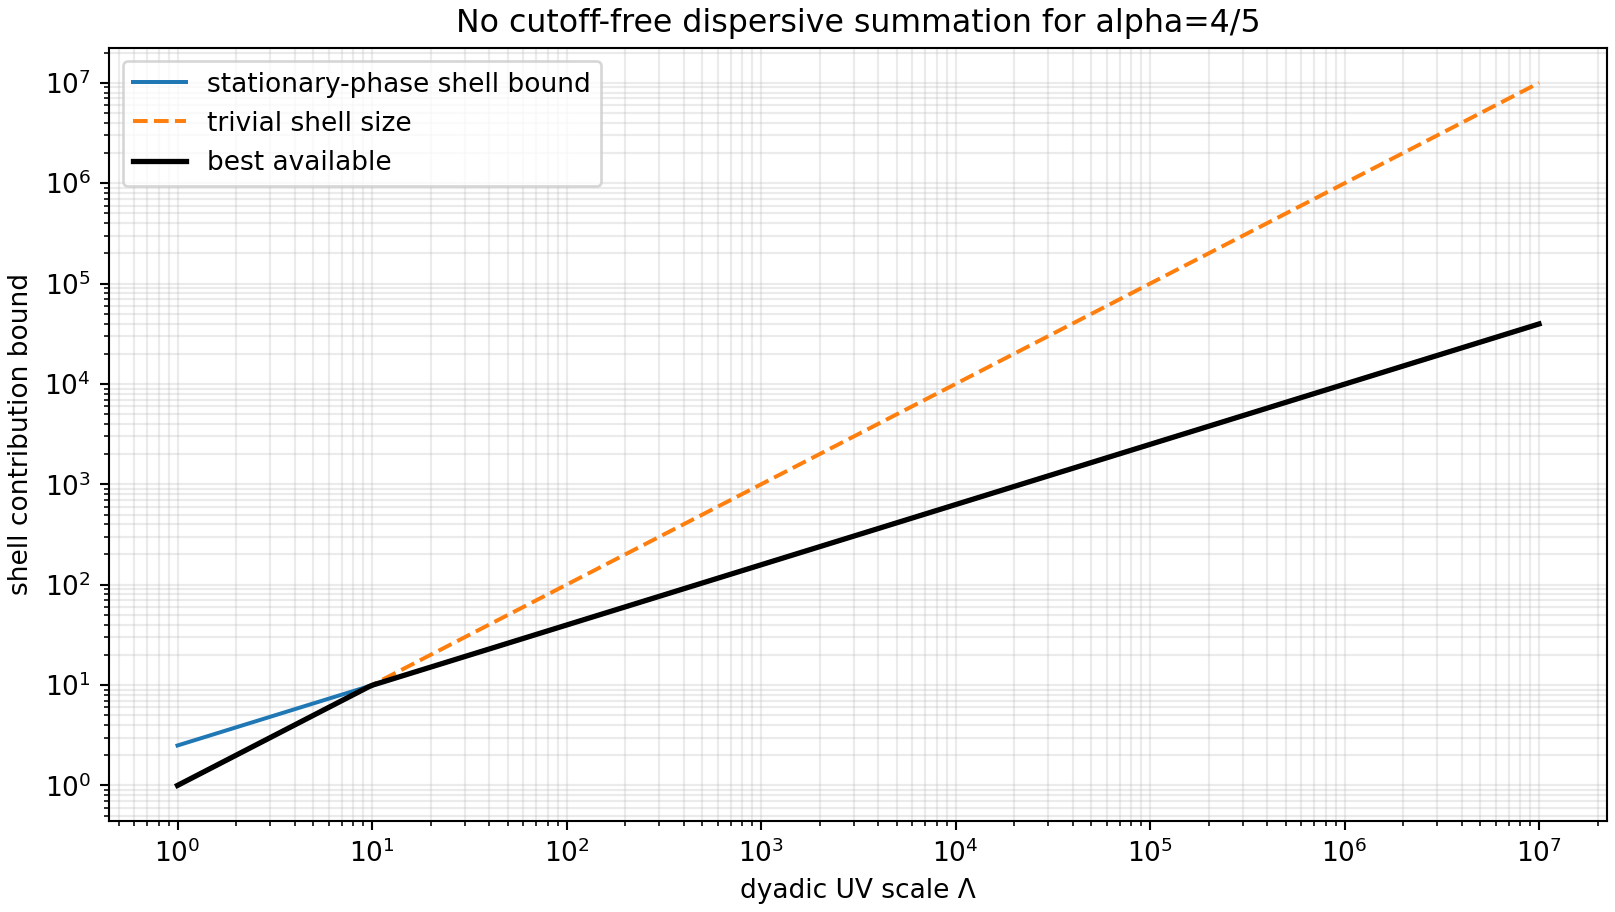
\includegraphics[width=0.94\textwidth]{FIN_Programs_125_137_Trace_Localizer_Physics_Figures/program129_fractional_wave_uv_obstruction.png}
\caption{The standard dyadic wave bound grows as \(\Lambda^{3/5}\) and is not ultraviolet summable.}
\end{figure}

The minimal mathematically safe object is therefore the cutoff family

\[
U_t^\Lambda
=
\mathbf1_{\{|q|\le\Lambda\}}
e^{-itC|q|^{4/5}},
\]

which is unitary on its cutoff subspace.

\textbf{Result:} \textbf{Proven obstruction for the standard cutoff-free dispersive route.}

This does not prove that every sophisticated distributional formulation or weighted estimate is impossible. It proves that the present operator alone does not supply a point detector and that the standard dyadic argument cannot remove the UV cutoff. Detector resolution is thus a genuine missing operational object, not a cosmetic detail.

\par\medskip\hrule\medskip

\chapter{Part IV --- Programs 130--132: physical calibration, apparatus learning, and flow}

\section{Program 130 --- The minimal dimensional calibration object}

\subsection{Construction}

Let \(x\) and \(t\) denote dimensionless lattice position and operational time. Introduce three positive calibration constants:

\[
\ell\quad\text{(length)},\qquad
\tau\quad\text{(time)},\qquad
\hbar\quad\text{(action)}.
\]

Then

\[
x_{\rm phys}=\ell x,
\qquad
t_{\rm phys}=\tau t,
\qquad
H_{\rm phys}=\frac{\hbar}{\tau}A.
\]

For the fractional generator,

\[
D_{4/5}=\frac{\ell^{4/5}}{\tau},
\qquad
c_H=\frac{\hbar\ell^{4/5}}{\tau}.
\]

\subsection{Rank theorem}

In logarithmic units, length, time, and energy depend on \((\log\ell,\log\tau,\log\hbar)\) through

\[
M=
\begin{pmatrix}
1&0&0\\
0&1&0\\
0&-1&1
\end{pmatrix}.
\]

Since

\[
\det M=1,
\qquad
\operatorname{rank}M=3,
\]

three independent calibrations are necessary to set those three physical dimensions.

\begin{figure}[htbp]
\centering
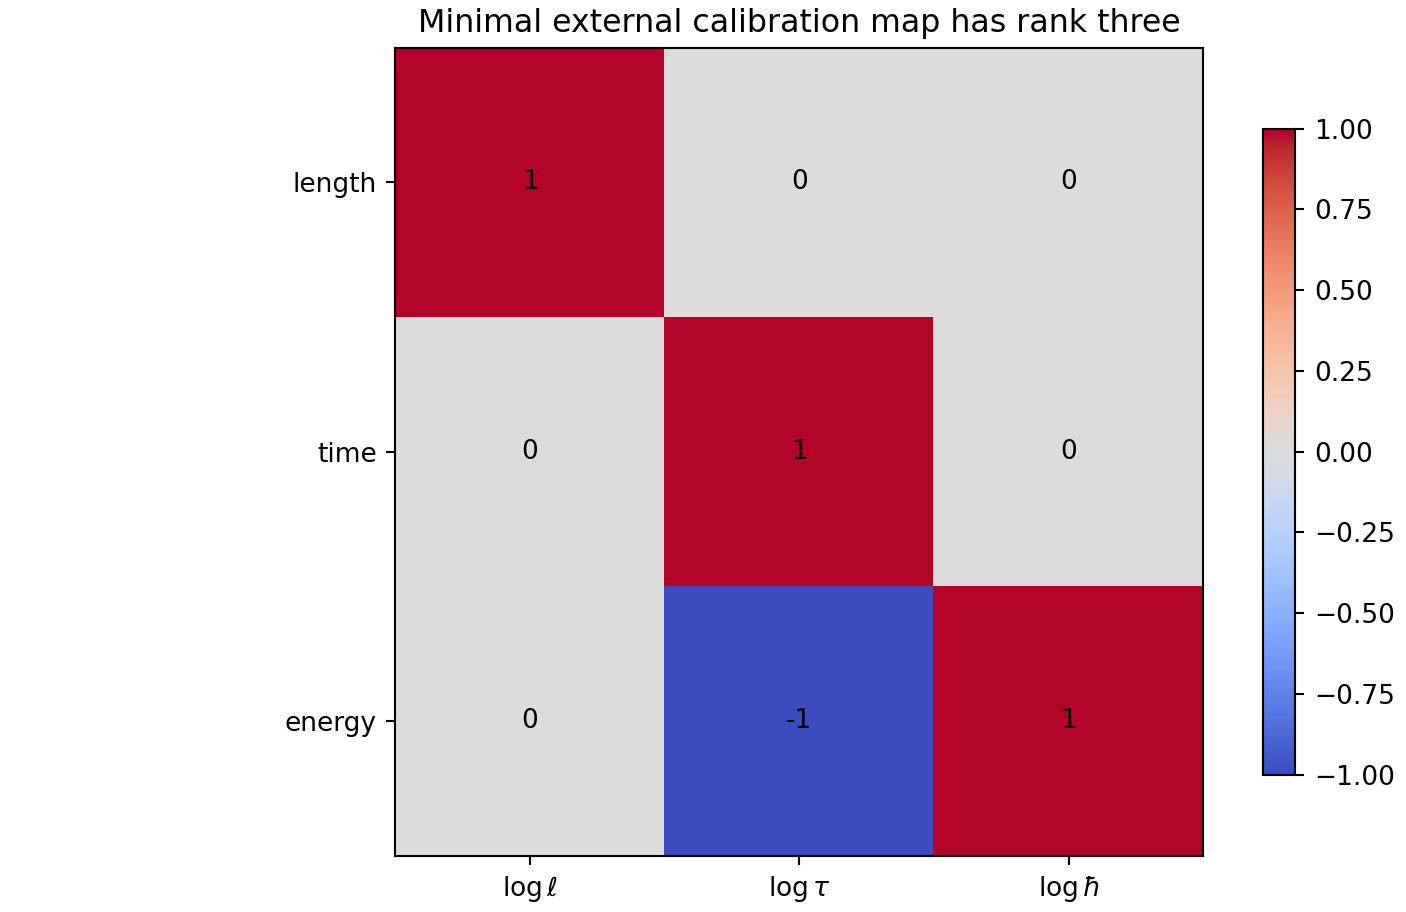
\includegraphics[width=0.94\textwidth]{FIN_Programs_125_137_Trace_Localizer_Physics_Figures/program130_dimensional_calibration.png}
\caption{The minimal physical calibration map has rank three.}
\end{figure}

With illustrative independent relative uncertainties of \(1\%\) in \(\ell\), \(2\%\) in \(\tau\), and \(3\%\) in \(\hbar\), linear error propagation gives

\[
\frac{\sigma_E}{E}=3.606\%,
\qquad
\frac{\sigma_{D_{4/5}}}{D_{4/5}}=2.154\%,
\qquad
\frac{\sigma_{c_H}}{c_H}=3.693\%.
\]

\textbf{Result:} \textbf{Proven dimensional-analysis theorem; conditional physical object constructed.}

No internal FIN theorem presently generates \(\ell,\tau,\hbar\). Spectral asymptotics can compare dimensionless scales, but without one dimensionful reference it cannot create SI length, duration, or action from pure numbers.

\section{Program 131 --- Nonparametric apparatus process tomography}

\subsection{Operational problem}

A measurement record is not determined by the system generator alone. An apparatus may have memory:

\[
\Pr(r_t\mid s_t,r_{<t})\ne\Pr(r_t\mid s_t).
\]

The smallest model-independent finite-memory approximation is a conditional table of order \(r\),

\[
\Pr(E_t\mid E_{t-r:t-1}),
\]

where \(E_t\) is the apparatus error bit.

\subsection{Synthetic identifiability test}

A reproducible synthetic channel was generated with refreshed error prevalence \(0.1\) and persistence \(0.8\). Orders zero, one, and two were fitted using Jeffreys-smoothed conditional frequencies. With 10,000 calibration records, held-out log losses per record are

\[
\begin{array}{c|ccc}
\text{order}&0&1&2\\
\hline
\text{log loss}&0.311244&0.119580&0.119683.
\end{array}
\]

The true order-one model is recovered. The order-two estimator approaches it but pays a finite-sample variance penalty.

\begin{figure}[htbp]
\centering
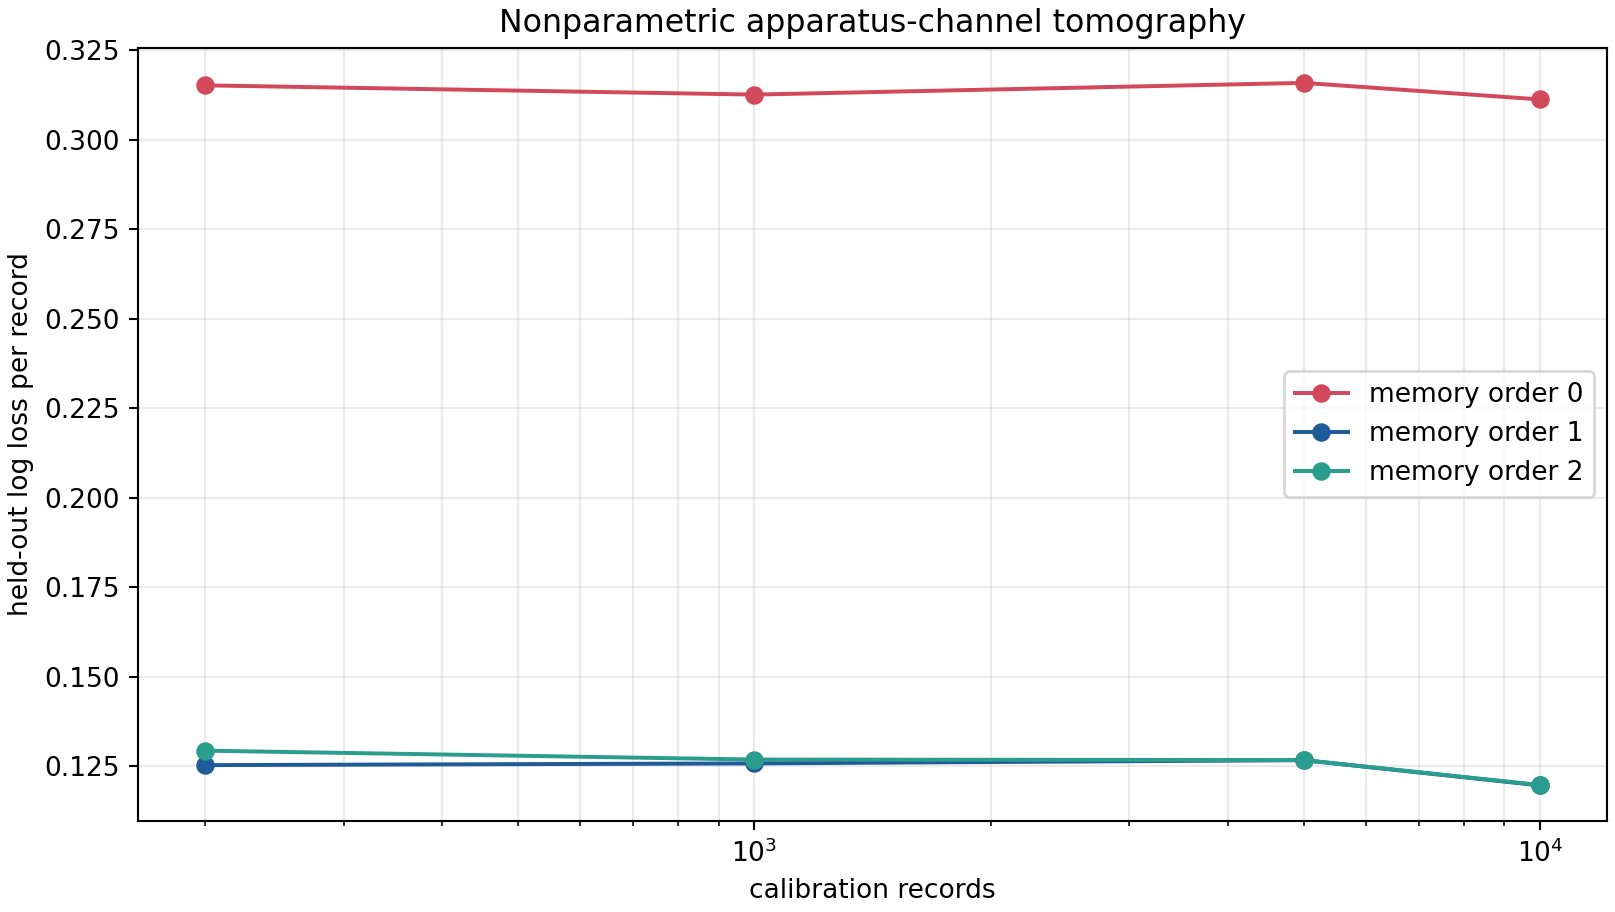
\includegraphics[width=0.94\textwidth]{FIN_Programs_125_137_Trace_Localizer_Physics_Figures/program131_apparatus_tomography.png}
\caption{Held-out log loss for nonparametric apparatus-memory models.}
\end{figure}

\textbf{Result:} \textbf{Constructed and numerically validated on synthetic data.}

The estimator supplies the missing mathematical type of a calibratable apparatus channel. It is not evidence that any physical apparatus follows FIN, and no external observations were used.

\section{Program 132 --- Exact projective crossover flow}

Consider the constructed crossover operator

\[
A_{\kappa,\nu}
=
\kappa(-\Delta)+\nu(-\Delta)^{2/5}.
\]

Let

\[
g=\frac{\nu}{\kappa}.
\]

Under length rescaling by \(b\), the ratio transforms as

\[
g(b)=b^{6/5}g.
\]

Compactify the positive ratio by

\[
x=\frac{g}{1+g}.
\]

Differentiation with respect to \(\log b\) gives the exact projective flow

\[
\frac{dx}{d\log b}
=
\frac65x(1-x).
\]

Its fixed points are \(x=0\), the local UV endpoint, and \(x=1\), the fractional IR endpoint. The crossover momentum is

\[
q_*=\left(\frac{\nu}{\kappa}\right)^{5/6}.
\]

\begin{figure}[htbp]
\centering
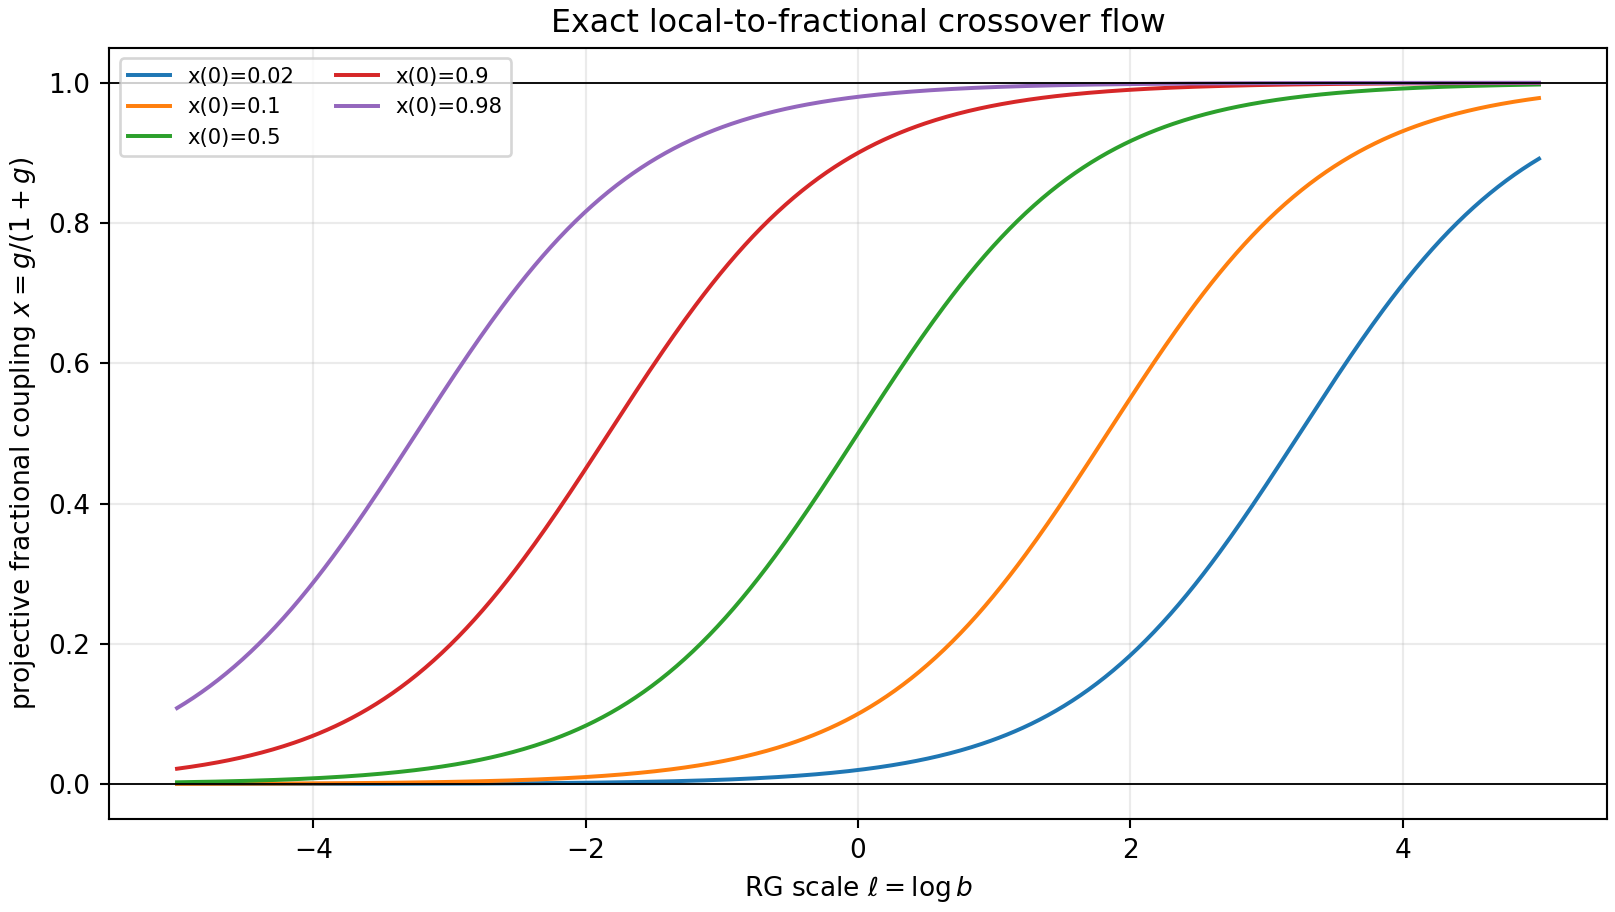
\includegraphics[width=0.94\textwidth]{FIN_Programs_125_137_Trace_Localizer_Physics_Figures/program132_crossover_rg_flow.png}
\caption{Exact projective flow from the local ultraviolet endpoint to the fractional infrared endpoint.}
\end{figure}

\textbf{Result:} \textbf{Proven for the constructed two-term operator.}

This is a scaling theorem, not a derivation of \(\kappa\) or \(\nu\) from strict FIN and not a full interacting renormalization group.

\par\medskip\hrule\medskip

\chapter{Part V --- Programs 133--136: parameter sources, bridge maps, and signed states}

\section{Program 133 --- Phase and frequency source falsification}

The new fibre object supplies several intrinsic integers:

\[
12,\ 5,\ 9,\ 17,\ 16,\ 4,\ 2,
\]

respectively carrier order, number of prime sectors, sum of dimensions, sum of squared dimensions, product of dimensions, number of real characters, and the \(p=3\) fibre dimension.

These integers reproduce the frozen phase and frequency exactly:

\[
\phi
=
\frac{17-4}{5\cdot16}
=
\frac{13}{80},
\]

\[
\omega
=
\frac{17(4\cdot12-4)-5}{5^3(2\cdot16)}
=
\frac{743}{4000}.
\]

The equalities are arithmetically correct. They are nevertheless not accepted as derivations.

\subsection{Uniqueness audit}

Within the limited template

\[
\frac{A-B}{CD},
\]

using the seven intrinsic integers, two ordered encodings reproduce \(\phi\). Within

\[
\frac{A(BC-B)-D}{D^3EP},
\]

four ordered encodings reproduce \(\omega\). Permutation equivalences already destroy literal uniqueness, while the much larger space of rational expressions contains indefinitely many target encodings.

Changing one input integer moves the results away from the frozen values. No functor, action, extremum, universality theorem, or robustness principle selects the displayed expressions.

\begin{figure}[htbp]
\centering
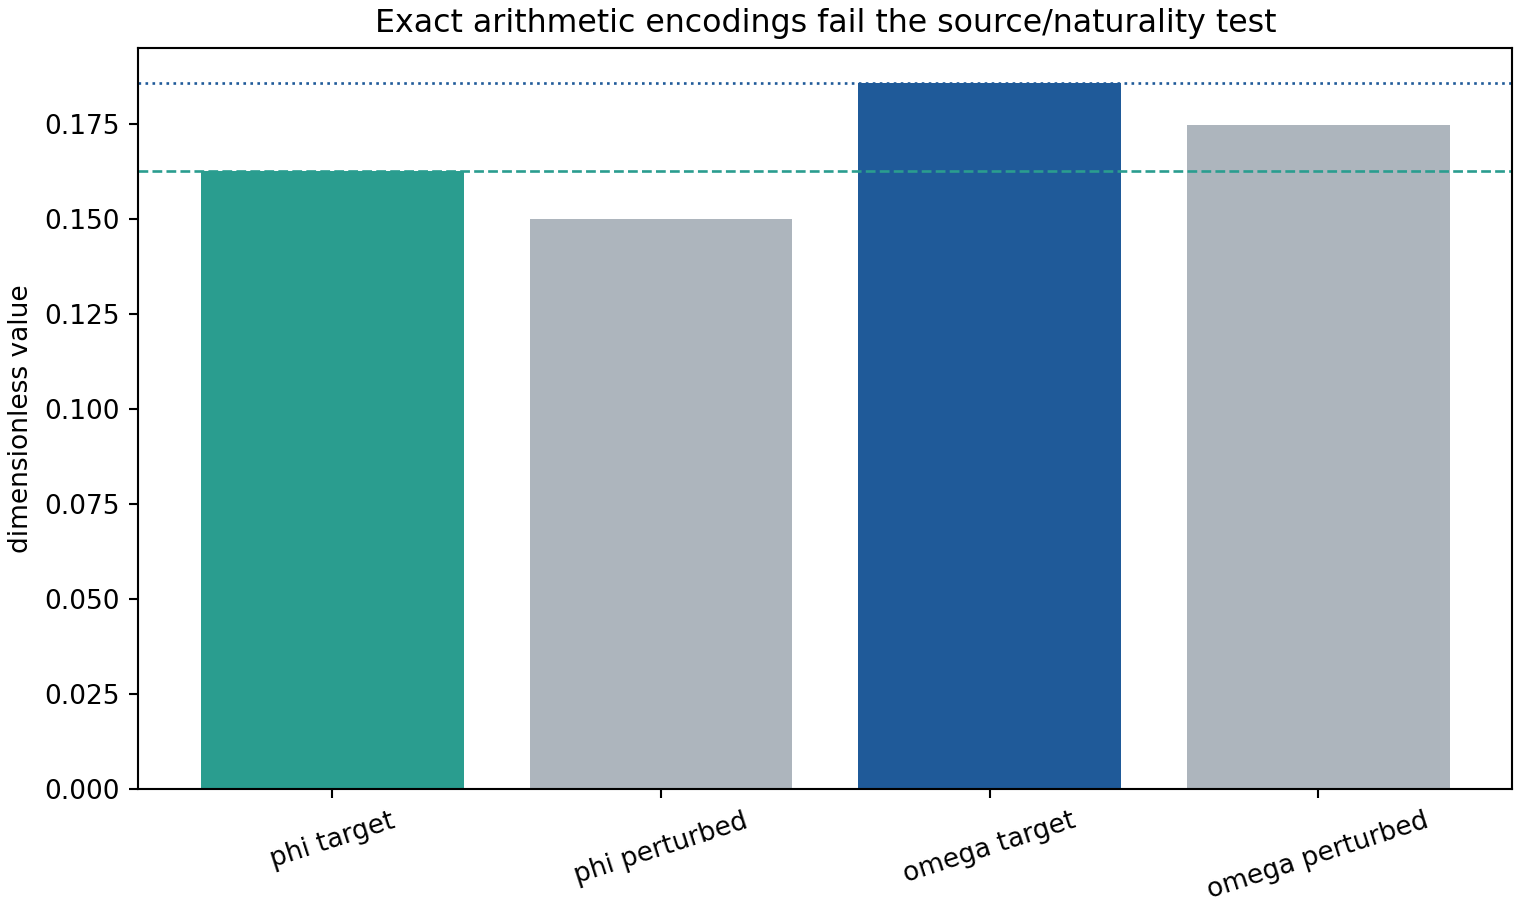
\includegraphics[width=0.94\textwidth]{FIN_Programs_125_137_Trace_Localizer_Physics_Figures/program133_phase_frequency_source_test.png}
\caption{Exact arithmetic parameter encodings fail robustness and source-selection tests.}
\end{figure}

\textbf{Result:} \textbf{Refuted as a source theorem.} Exact post-hoc arithmetic is reported as an identity, not promoted to physics.

\section{Program 134 --- Amplitude projectivization}

Define the amplitude quotient

\[
\Pi_0(K)=\frac{K}{K(0)},
\qquad K(0)\ne0.
\]

It satisfies

\[
\Pi_0(cK)=\Pi_0(K),
\qquad
\Pi_0(\Pi_0(K))=\Pi_0(K).
\]

Thus \(\alpha_{\rm geo}\) disappears from the projectivized legacy shape. However, over distances \(0\le d\le64\), the relative \(L^2\) mismatch between projectivized legacy and strict shapes is

\[
3.70714.
\]

Even the best scalar-only fit has relative residual

\[
0.933864.
\]

\begin{figure}[htbp]
\centering
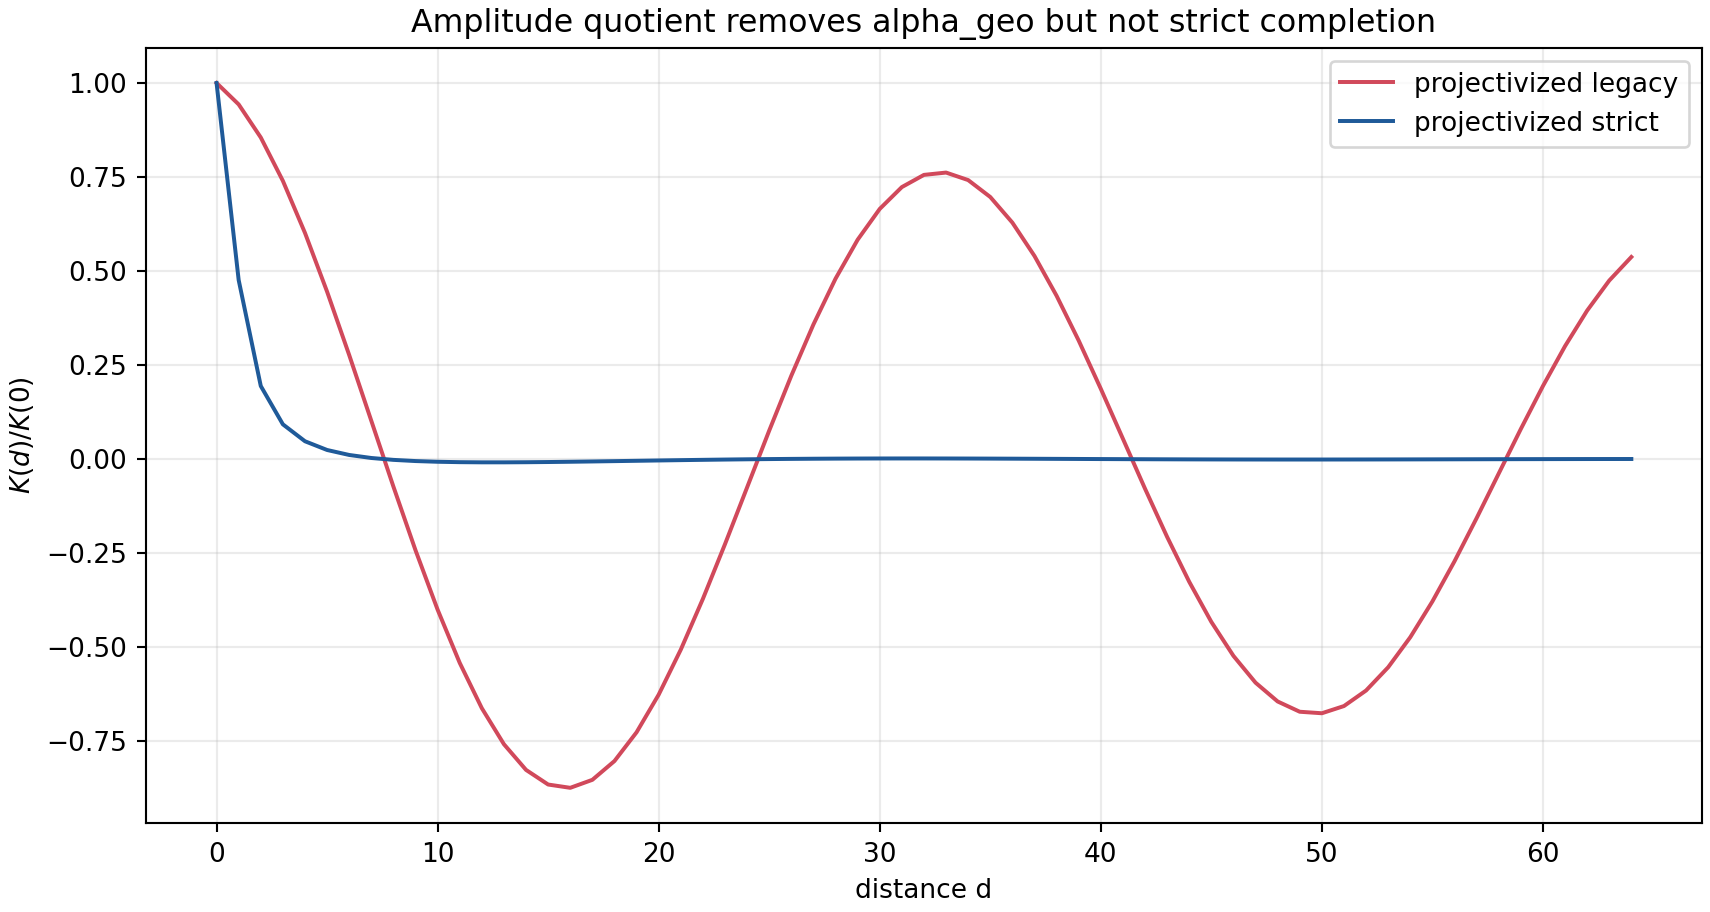
\includegraphics[width=0.94\textwidth]{FIN_Programs_125_137_Trace_Localizer_Physics_Figures/program134_amplitude_projectivization.png}
\caption{Amplitude projectivization removes \(\alpha_{\rm geo}\) but leaves a large shape mismatch.}
\end{figure}

\textbf{Result:} \textbf{Proven quotient theorem and strong finite falsification of scalar-only completion.}

The quotient clarifies one legitimate sense in which amplitude can be gauge-like for kernel shape. It also proves a role-transfer obstruction: absolute-amplitude observables are erased by \(\Pi_0\) and cannot be transported through this map alone.

\section{Program 135 --- Conditional damping-side bridge}

Expose the unresolved trace weight rather than hiding it:

\[
\eta(w)=2-w_2.
\]

The trace-parameterized damping factor mapping the legacy denominator to the strict denominator is

\[
D_w(d)
=
\frac{1+\beta_{\rm tors}d}
{1+d^{2-w_2}}.
\]

If the uniform sector state is added, \(w_2=1/5\) and

\[
D_{\rm unif}(d)
=
\frac{1+\beta_{\rm tors}d}
{1+d^{9/5}}.
\]

The numerical reconstruction residual is exactly zero to floating-point evaluation because the same algebraic expression is evaluated on both sides.

The nonzero monomial tail

\[
T(d)=\beta d^\eta
\]

is multiplicative only if

\[
T(ab)=T(a)T(b)
\quad\Longrightarrow\quad
\beta=1.
\]

For the uniform trace, dyadic retention is

\[
2^{1-\eta}
=
2^{-4/5}
=
e^{-\alpha_{\rm geo}/5}.
\]

\begin{figure}[htbp]
\centering
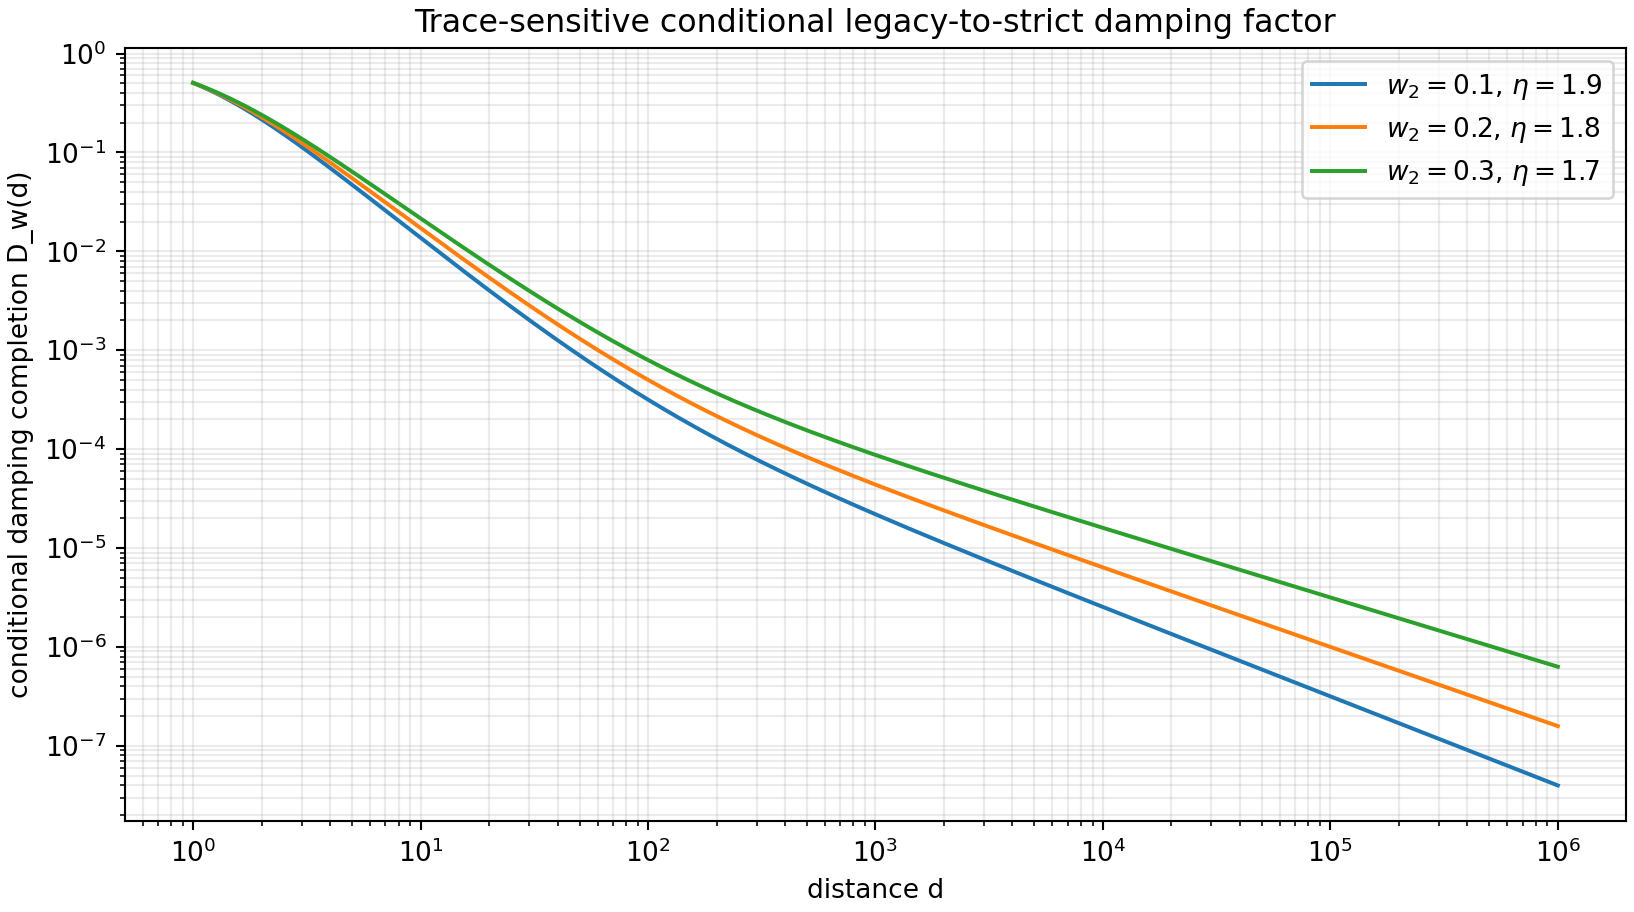
\includegraphics[width=0.94\textwidth]{FIN_Programs_125_137_Trace_Localizer_Physics_Figures/program135_conditional_damping_bridge.png}
\caption{The trace-dependent family of conditional damping completion factors.}
\end{figure}

\textbf{Result:} \textbf{Exact but conditional.}

Program 125 prevents promotion to a strict theorem: the uniform sector state is not forced. The phase and frequency source, amplitude-role semantics, and strict coupling theorem also remain absent. This is a damping-side completion factor, not a full bridge and not a role-transfer theorem.

\section{Program 136 --- A signed operational state receiver}

Let \(A\) be the fractional circulant on \(C_{12}\) with eigenvalues \(|q|^{4/5}\). For a density matrix \(\rho\), define the nearest-link signed receiver

\[
\Lambda(\rho,A)
=
2\,\operatorname{Im}
\sum_{i=0}^{11}
\rho_{i,i+1}A_{i+1,i}.
\]

Prepared Fourier branches give

\[
\Lambda(\rho_{+1},A)=+0.498004,
\qquad
\Lambda(\rho_{-1},A)=-0.498004,
\]

and

\[
\Lambda(\rho_{+2},A)=+0.862568,
\qquad
\Lambda(\rho_{-2},A)=-0.862568.
\]

The reflection-invariant \(k=0\) state and the thermal state \(f(A)\) give zero.

\begin{figure}[htbp]
\centering
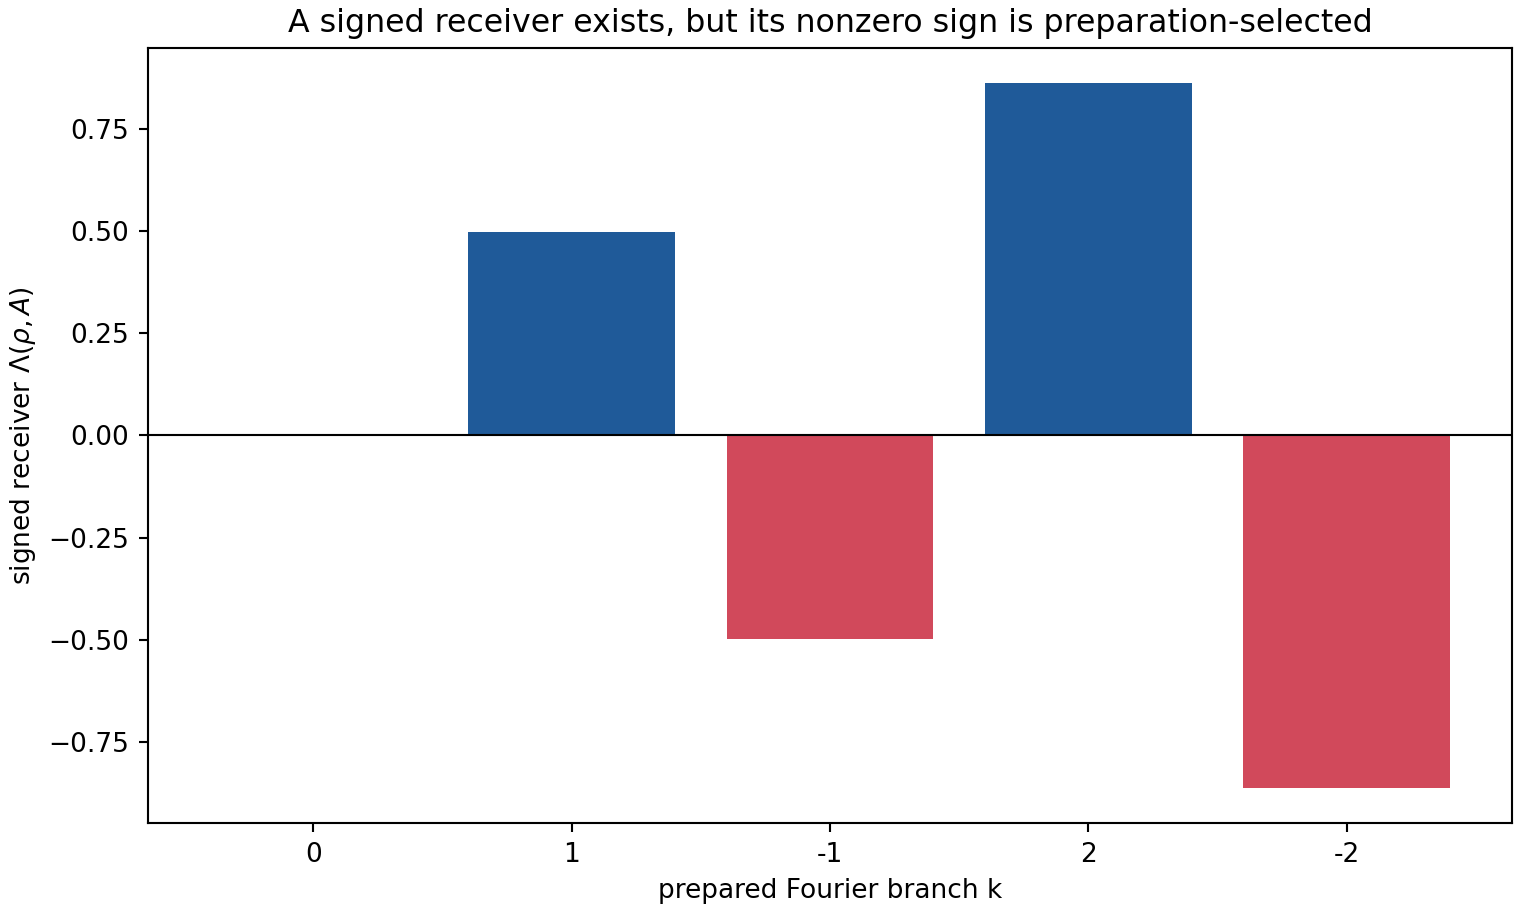
\includegraphics[width=0.94\textwidth]{FIN_Programs_125_137_Trace_Localizer_Physics_Figures/program136_signed_state_receiver.png}
\caption{The signed receiver distinguishes prepared opposite branches but does not choose a branch.}
\end{figure}

\textbf{Result:} \textbf{Constructed and proven sign-paired.}

This object is a receiver, not a source. It reads orientation after the preparation chooses \(k\) or \(-k\). Reflection symmetry pairs the two branches, so no non-premise preparation law is obtained. QW-2191 is not discharged.

\par\medskip\hrule\medskip

\chapter{Part VI --- Program 137, integrated conclusions, and falsification ledger}

\section{Program 137 --- External-data audit}

Five local data-intake or preregistration JSON artifacts were scanned for explicit positive admission markers. No artifact admits external data. The present round uses repository-internal values and reproducible synthetic records only.

\textbf{Result:} \textbf{Reproducible local audit.}

This is not a forensic scan of every repository byte. It is sufficient to state that no external dataset entered the explicit research-chain intake mechanism used by these releases.

\section{Newly constructed theoretical objects}

The round constructs the following objects without claiming more than their types support.

\begin{enumerate}
\item 
A presentation-independent homological--character localizer on \(C_{12}\).

\item 
The enlarged-symmetry trace simplex and the carrier-natural full simplex on the five-sector algebra.

\item 
A continuous finite-window enclosure of the fractional symbol.

\item 
Quantitative finite-step characteristic-function intervals.

\item 
A UV-cutoff fractional wave family.

\item 
A rank-three dimensional calibration map.

\item 
A nonparametric finite-memory apparatus process tensor.

\item 
An exact projective local-to-fractional crossover flow.

\item 
An amplitude-projective kernel quotient.

\item 
A trace-parameterized damping completion family.

\item 
A signed state-dependent current receiver.

\end{enumerate}

\section{Falsification ledger}

\subsection{\texorpdfstring{"The fibre dimensions canonically imply \(9/5\)"}{"The fibre dimensions canonically imply 9/\allowbreak{}5"}}

\textbf{Refuted.} They imply an affine readout \(\eta=2-w_2\). The state \(w\) is additional. The invariant state space is not a point.

\subsection{"The normalized Hilbert trace supplies the missing choice"}

\textbf{Refuted for \(9/5\).} It supplies \(17/9\).

\subsection{"The fibre object is presentation-dependent numerology"}

\textbf{Refuted at the \(C_{12}\) carrier level.} The multiplication maps, kernel homology, and character representation are natural under cyclic-group isomorphisms.

\subsection{"The fractional law was seen only at selected frequencies"}

\textbf{Substantially weakened.} Every cell in a finite compact window is enclosed. Formal interval arithmetic and a true \(q\to0\) rate remain open.

\subsection{"The same operator automatically defines a pointwise wave experiment"}

\textbf{Refuted by the present route.} The unitary \(L^2\) group exists, but the standard UV shell estimate is nonsummable. Detector bandwidth is necessary.

\subsection{"Dimensionless mathematics can choose physical units internally"}

\textbf{Refuted without a new dimensionful source.} The minimum calibration map has rank three.

\subsection{"The exact rational encodings derive phase and frequency"}

\textbf{Refuted.} They are target-dependent identities without a selection theorem.

\subsection{"Amplitude normalization completes legacy to strict"}

\textbf{Refuted.} Projective shape mismatch remains large, and amplitude-dependent roles are erased.

\subsection{"A signed detector is a strict selector"}

\textbf{Refuted.} Opposite prepared branches give opposite signs. The missing object is the branch-preparation law.

\section{Theoretical architecture after Program 137}

The smallest honest architecture now has four layers:

\[
\begin{gathered}
\boxed{\text{strict carrier and operator}}
\\ \downarrow \\
\boxed{\text{natural localizer plus chosen state}}
\\ \downarrow \\
\boxed{\text{operational process and apparatus}}
\\ \downarrow \\
\boxed{\text{physical calibration and data}}.
\end{gathered}
\]

The first layer is repository-internal. Part of the second layer---the localizer---is now constructed, while its distinguished state remains open. The dimensionless part of the third layer is constructible; its preparation and detector-resolution sources remain conditional. The fourth layer is external until physical standards and observations are supplied.

The missing theorem is therefore narrower than "derive all physics from the spectral theorem." It would have to do at least three nontrivial things:

\begin{enumerate}
\item 
select a distinguished state on the localized sector algebra;

\item 
induce a non-premise preparation/\allowbreak{}orientation law compatible with that state;

\item 
connect dimensionless spectral scales to a calibrated physical standard.

\end{enumerate}

No theorem established here simultaneously performs those tasks.

\section{Research assessment}

\subsection{Proven}

\begin{itemize}
\item 
enlarged-symmetry invariant traces form the stated two-simplex, while carrier naturality alone leaves the full simplex;

\item 
\(9/5\) is not selected by invariance;

\item 
the Hilbert trace gives \(17/9\);

\item 
the fibre localizer is presentation-independent on \(C_{12}\);

\item 
the cutoff fractional wave family is well-defined in \(L^2\);

\item 
the standard UV curvature bound is nonsummable;

\item 
the physical calibration matrix has rank three;

\item 
the projective crossover beta function is exact;

\item 
amplitude projectivization is idempotent and cannot preserve amplitude-dependent roles;

\item 
the signed receiver is paired under orientation reversal.

\end{itemize}

\subsection{Strong evidence}

\begin{itemize}
\item 
the \(4/5\) symbol law holds with at most the stated conservative relative remainder across the finite frequency window;

\item 
the finite-step stable comparison has the reported numerical bounds;

\item 
nonparametric apparatus memory is identifiable in the synthetic test.

\end{itemize}

\subsection{Conditional}

\begin{itemize}
\item 
\(\eta=9/5\) from the uniform sector state;

\item 
\(\beta=1\) from a nonzero multiplicative monomial tail;

\item 
the damping-side completion map;

\item 
physical predictions after \((\ell,\tau,\hbar)\) calibration;

\item 
pointwise wave records after detector-bandwidth specification.

\end{itemize}

\subsection{Open}

\begin{itemize}
\item 
a strict distinguished sector state;

\item 
a strict phase/\allowbreak{}frequency source;

\item 
a strict non-premise orientation preparation;

\item 
a full legacy-to-strict completion certificate;

\item 
a role-transfer theorem;

\item 
an internal dimensionful reference;

\item 
external experimental validation.

\end{itemize}

\par\medskip\hrule\medskip

\chapter{Part VII --- Recommended Programs 138--150}

The next studies are ranked to avoid replaying closed lanes. Each introduces a new typed object or a genuinely stronger validation standard.

\section{Program 138 --- Modular-state selection on the fibre algebra}

Construct a faithful state \(\rho\) on a noncommutative enlargement of \(\mathcal A_{\mathcal F}\) and test whether a KMS or modular invariance condition selects \(w_2=1/5\). The falsification criterion is strict: if the modular Hamiltonian must be chosen to encode the desired weights, no source has been found.

\textbf{Probability of useful result:} 0.55.\\
\textbf{Probability of uniquely deriving \(9/5\):} 0.15.

\section{Program 139 --- Maximum-entropy reference-measure theorem}

Classify all reference measures and constraint sets for which the maximum relative-entropy state on the five sectors is uniform. Determine whether any reference measure is generated naturally by the localizer rather than inserted. This program should state a no-go theorem if uniformity is merely a choice of counting measure.

\textbf{Probability of useful result:} 0.85.\\
\textbf{Probability of strict trace closure:} 0.25.

\section{Program 140 --- Morita-stability test of the exponent readout}

Replace the fibre algebra by matrix amplifications and Morita-equivalent presentations. Test whether \(\eta(w)\) survives canonical equivalence. If the uniform-sector trace changes under amplification while the physical exponent is meant to remain fixed, the current readout is not categorical enough.

\textbf{Probability of useful result:} 0.80.

\section{Program 141 --- Validated-FFT interval certificate}

Recompute Program 127 using outward-rounded interval arithmetic or a validated FFT. Produce a formally checkable enclosure on the entire window. This is the highest-priority proof upgrade because it turns strong numerical evidence into a computer-assisted theorem.

\textbf{Probability of success:} 0.90.

\section{Program 142 --- Diophantine oscillatory-tail rate}

Use explicit rational-approximation bounds for \(\omega/(2\pi)=743/(8000\pi)\) to control oscillatory tail averages and derive an actual remainder rate in

\[
S(q)=C|q|^{4/5}+R(q).
\]

The target is a bound \(|R(q)|\le C'|q|^{4/5+\delta}\) or a proof that the available arithmetic information cannot yield any uniform \(\delta>0\).

\textbf{Probability of a useful bound:} 0.45.

\section{Program 143 --- Weighted dispersive estimates}

The cutoff-free unweighted route failed. Test whether weighted Sobolev, Besov, or frequency-localized estimates define operationally meaningful wave records without a hard UV cutoff. The detector norm must be specified before the estimate is evaluated.

\textbf{Probability of useful partial theorem:} 0.70.\\
\textbf{Probability of removing all resolution data:} 0.10.

\section{Program 144 --- Detector-resolution renormalization}

Construct a detector response \(R_\sigma\) and study

\[
\mathcal M_{\sigma,t}=R_\sigma U_t.
\]

Derive how predictions change as \(\sigma\to0\) and identify which observables have a finite resolution-independent limit. This turns the UV obstruction into a measurable apparatus parameter.

\textbf{Probability of success:} 0.85.

\section{Program 145 --- Joint system--instrument identifiability}

Extend Program 131 from a known synthetic system to simultaneous estimation of the fractional generator and a memory channel. Derive conditions under which generator changes cannot be absorbed into apparatus memory.

\textbf{Probability of useful result:} 0.80.

\section{Program 146 --- Calibration-invariant observable ratios}

Search systematically for combinations of records in which \(\ell,\tau,\hbar\) cancel. Rank those ratios by sensitivity to the fractional exponent and robustness to apparatus memory. Such quantities are the shortest route to falsifiable dimensionless tests.

\textbf{Probability of success:} 0.90.

\section{Program 147 --- Preparation-resource theory for the sign torsor}

Treat \(k\) versus \(-k\) preparation as a resource. Classify free reflection-symmetric operations and monotones for signed preparation. Prove whether a nonzero \(\Lambda\) can be generated from symmetric states under the allowed strict operations.

\textbf{Probability of a no-go theorem:} 0.85.\\
\textbf{Probability of finding an internal selector:} 0.15.

\section{Program 148 --- Coupled state--damping variational principle}

Construct the smallest convex functional of a sector state \(w\) and a damping profile \(D\) whose Euler equations could select both. The action must be target-free and invariant under the admitted carrier symmetries. An after-the-fact term minimized at \(w_2=1/5\) is disallowed.

\textbf{Probability of useful obstruction:} 0.75.\\
\textbf{Probability of unique strict selection:} 0.20.

\section{Program 149 --- Full completion-map commutative diagram}

Assemble amplitude quotient, trace-dependent damping, phase/\allowbreak{}frequency data, and certified topological information into a typed diagram. Mark every arrow as strict, conditional, quotient, or absent. Prove which diagrams commute and which cannot commute because amplitude roles are lost.

\textbf{Probability of useful result:} 0.95.

\section{Program 150 --- Pre-data physical protocol and rejection thresholds}

Write one executable protocol specifying preparation, environment, clock, detector response, calibration, record format, null model, alternative, test statistic, and rejection region before any external data are admitted. Focus on calibration-invariant ratios from Program 146.

\textbf{Probability of producing a valid preregistration:} 0.90.\\
\textbf{Probability of near-term empirical execution:} dependent on apparatus and dataset availability.

\section{Priority order}

The recommended execution order is

\[
141\to139\to140\to146\to144\to145\to147\to148\to149\to150,
\]

with Programs 138, 142, and 143 run as higher-risk mathematical branches.

The rationale is:

\begin{itemize}
\item 
first formalize the strongest numerical result;

\item 
then decide whether the trace can be selected without circularity;

\item 
next identify unit-free observables and detector resolution;

\item 
only then couple system and apparatus or prepare an empirical protocol.

\end{itemize}

\par\medskip\hrule\medskip

\chapter{Reproducibility statement}

The executable research file is

fin\_programs\_125\_137\_trace\_localizer\_physics.py.

Machine-readable results are stored in

FIN\_Programs\_125\_137\_Trace\_Localizer\_Physics\_Results.json.

Thirty-five regression tests are stored in

test\_fin\_programs\_125\_137\_trace\_localizer\_physics.py.

Twelve figures were generated from the same executable. Randomized synthetic apparatus calculations use seed 20260727. No external dataset is admitted.

\chapter{Conclusion}

Programs 125--137 sharpen the physical interpretation of FIN by separating three objects that had been in danger of conflation:

\[
\text{localizer},\qquad
\text{state on localized sectors},\qquad
\text{physical calibration}.
\]

The localizer can be constructed naturally. The state is not selected by symmetry and is not rescued by the normalized Hilbert trace. Physical calibration remains an independent rank-three interface. The fractional operator itself is mathematically productive: it supports stable diffusion, unitary wave evolution, an exact crossover flow, and operational receiver models. But wave measurements require resolution, signed receivers require signed preparation, and dimensional predictions require standards.

The most defensible mathematical interpretation after falsification is therefore not that one spectral operator already constitutes a physical universe. It is that FIN supplies a dimensionless fractional spectral generator on a finite informational carrier, together with a natural localization structure. Turning that structure into physics requires a distinguished state, a preparation/\allowbreak{}instrument law, dimensional calibration, and external records. Those are now explicit mathematical obligations rather than unnamed gaps.

\chapter{Selected references}

\begin{enumerate}
\item 
W. Feller, \emph{An Introduction to Probability Theory and Its Applications, Volume II}, Wiley.

\item 
K. Sato, \emph{Lévy Processes and Infinitely Divisible Distributions}, Cambridge University Press.

\item 
D. Applebaum, \emph{Lévy Processes and Stochastic Calculus}, Cambridge University Press.

\item 
R. Schilling, R. Song, and Z. Vondracek, \emph{Bernstein Functions}, De Gruyter.

\item 
E. M. Stein, \emph{Harmonic Analysis}, Princeton University Press.

\item 
S. Mac Lane, \emph{Categories for the Working Mathematician}, Springer.

\item 
J.-P. Serre, \emph{Linear Representations of Finite Groups}, Springer.

\item 
M. Nielsen and I. Chuang, \emph{Quantum Computation and Quantum Information}, Cambridge University Press.

\item 
F. G. S. L. Brandão and G. Gour, "Reversible framework for quantum resource theories," \emph{Physical Review Letters} 115, 070503.

\item 
J. Pearl, \emph{Causality}, Cambridge University Press.

\end{enumerate}

\chapter{Suggested citation}

\.Zuchowski, K. (2026). \emph{FIN Programs 125--137: Trace Selection, Natural Localizers, Fractional Physics, and Operational Sources} (FIN Research Monograph, Release 10.13; Version 1.0.0) [Preprint]. Zenodo.


\clearpage
\chapter*{Archival note}
\addcontentsline{toc}{chapter}{Archival note}
Machine-readable results are stored in
\path{FIN_Programs_125_137_Trace_Localizer_Physics_Results.json}.
The executable, thirty-five tests, and twelve generated figures reproduce the
release.

\medskip
\noindent\textbf{Suggested citation:}

\.Zuchowski, K. (2026). \emph{FIN Programs 125--137: Trace Selection,
Natural Localizers, Fractional Physics, and Operational Sources}
(FIN Research Monograph, Release 10.13; Version 1.0.0) [Preprint]. Zenodo.
\end{document}
